
\section{Experimental Evaluation}
\label{sec:experiments_lifelong}

In this section, we will test POLIS against different baselines in a set of lifelong \gls{rl} tasks.
The first set of experiments will consider an undelayed non-stationary environment to evaluate the ability of the algorithms to face changing dynamics. 
Then, a second set of experiments will consider adding some delay to previous tasks to assess the robustness of POLIS against delay.
Throughout this section, we will make an assumption on the particular cases of \glspl{mdp} that we will be interested in for lifelong \gls{rl}. 
The assumption is that the agent cannot influence part of the state by its actions and that only this part of the state can be non-stationary. 
This is, for instance, a common assumption in financial mathematics to simplify the analysis. 
It is usually assumed that trading only a small investment size does not influence the market dynamics.
This greatly simplifies the experimental setup and allows one to evaluate more clearly the abilities of our algorithm against an observable non-stationarity. 
The assumption is formally displayed below.
\begin{ass}
	\label{ass:factorable_state}
The transition model $\markovchaintransition= (\markovchaintransition_t)_{t \in \naturalnumbers}$ factorises as follows, for every $x = (x^c,x^u) \in \statespace$, $a \in \actionspace$, and $t \in \naturalnumbers$:
\begin{equation}
	\markovchaintransition_t(x'\vert x,a) = \markovchaintransition^c({x'}^c\vert x^c,x^u,a) \markovchaintransition_t^u({x'}^u\vert x^u) .
\end{equation}
\end{ass}

In addition to this assumption, in the task that we consider below, $\markovchaintransition^c$ is deterministic. 
This allows getting the value of the $\alpha$-step behind the expected return by sampling the controllable part of the state with a new policy while the non-stationary part of the state $x^u$ remains fixed. 
Therefore, we have access to the exact value of the gradient of the $\alpha$-step behind the expected return without requiring importance sampling. 

Next, we describe the setting of the experiments in \Cref{subsec:setting_exp_lifelong} before providing the results in \Cref{subsec:results_lifelong}. 


\subsection{Setting}
\label{subsec:setting_exp_lifelong}


\subsubsection{Tasks}
First, we describe the general context of lifelong learning. 
The schedule of a lifelong interaction with an environment can be divided into two periods. 
In the first period, which we call the \emph{behavioural period}, a behavioural hyper-policy samples data from the environment. 
This is necessary to collect enough data to compute the first {$\alpha$-step behind expected return} used in our surrogate objective.
Then, in the second period, the agent continues to interact with the environment from the point where the behavioural hyper-policy left it. However, it can now retrain its hyper-policy periodically.
In practice, we retrain every 50 steps in all tested environments.
Each time, 100 steps of the gradient are made.
We refer to this period as the \emph{target period}.
For all tasks, we set $\gamma=\omega=1$.

\noindent\textbf{Undelayed EUR-USD Trading.}\indent The first task is similar to the Trading task in \Cref{subsubsec:tasks_imitation}. 
It also considers the trading of the EUR-USD (\texteuro/\$) currency pair on Forex, but this time on a daily basis.
The agent can choose a continuous action in $[-1,1]$; $1$ and $-1$ correspond to buy or sell with the maximum order size of 100k\$ USD, while action $0$ corresponds to staying flat.
Placing ourselves under \Cref{ass:factorable_state}, we assume that the maximum order size is small compared to the available market liquidity and therefore has no impact on market dynamics.
The state observed by the agent is composed of its current portfolio ($x_{t}^{c}$), that is, exactly the value of its previous action and the current exchange rate of the currency ($x_{t}^{u}$).
We divide historical data into three datasets, 2009-2012, 2013-2016, and 2017-2020; each period has a little more than $1000$ data points.
Historical rates for the period are given in \Cref{subsubsec:datasets_lifelong}.
The reward is defined as $r_{t}=a_t(x_{t+1}^{u}-x_{t}^{u})-f\lvert a_t - x_{t}^{c}\rvert$ where $f$ is a fee which amounts to $1\mathrm{e}{-3}\;\%$ of the investment size.
We set $\alpha$ at 500 and also consider a target period of 500 steps.
It is important to note that, since there are no clear distinctions between training and testing in the lifelong framework, selecting hyperparameters (referring to POLIS parameters, not the hyper-policy) can be complex.
Selecting the best hyperparameters by evaluating the performance on the target period is dangerous as it would obviously overfit and generalise badly if, for example, the target period was extended.
To study this problem, we compare two hyperparameter selection schemes for this task.
For the first, we select hyperparameters on the target period for the dataset 2009-2012 and evaluate them on the other two datasets.
In the second approach, we both select the hyperparameters and evaluate on the target period of the last two datasets.

\noindent\textbf{Undelayed Vasicek Trading.}\indent Because the EUR-USD currency pair is a highly complex asset, we consider the trading of a synthetic rate with smoother non-stationary in order to provide a better signal-to-noise ratio to the agents.
We preserve the overall trading framework and only modify the exchange rate $(x_{t}^{c})_{t\ge0}$ where we substitute a Vasicek process for the historical EUR-USD rates. 
The rest of the framework remains the same. 
The considered Vasicek process is $x_{t+1}^{c} = 0.9 x_{t}^{c} + u_t$, where $u_t\sim\mathcal{N}(0,1)$. 

\noindent\textbf{Undelayed Dam.}\indent This third task considers a water resource management problem, in which a dam is used to control the level of a lake.
The lake gets water from some inflows (e.g. rainwater) while the dam controls its outflows. 
The goal is to satisfy a certain demand (e.g. a town's water supply) with outflowing water, even in drought periods. 
This involves saving rainwater in anticipation while avoiding flooding.
We use the environment model from \cite{castelletti2010tree, pmlr-v80-tirinzoni18a}.
Three different stochastic yearly inflows are considered\footnote{Their means are given in \Cref{subsubsec:datasets_lifelong}}.
The agent has no impact on them, satisfying \Cref{ass:factorable_state}.
As a state, the agent observes the level of the lake for the current day.
The only modification to the original setting of \cite{castelletti2010tree, pmlr-v80-tirinzoni18a} is that the agent does not observe the day of the year to ensure non-stationarity.
Otherwise, the agent can learn to map the day of the year to its expected inflow, and this casts the problem back into stationarity.
The action space is continuous. 
We consider a flooding level of $F=300$ and a daily demand for water of $D=10$.
For some lake level $x$ and some selected out-flow--or action--$a$, a penalty of $c_D = (\max(a-D,0))^2$ is collected for not meeting the demand while an extra penalty of $c_F = (\max(x-F,0))^2$ is added for flooding.
The total cost combines these penalties depending on the inflow profile by weighting the two costs as detailed in \Cref{subsubsec:datasets_lifelong}. 
To better grasp the process's dynamics, we set $\alpha$ to 1000 so that enough years of past data are used inside the estimator. 
We set the target period's length to 500 steps. 
Concerning hyperparameters, it appears that for this environment the results are less sensitive to the choice of hyperparameters, we, therefore, select them on the first inflow profile only.
% AS we will see in the results, it may be necessary to change the frequency of retraining to have longer periods without updates in order to amplify the necessity to adapt to non-stationary. 

\noindent\textbf{Delayed Vasicek Trading.}\indent This task is the same as the previous Vasicek trading one with the addition of a delay.
We consider delays $\delay$ in the range $[\![1,10]\!]$ to study the impact of increasing delay on return. 
As explained throughout this chapter, here the agent is memoryless. 
Seeing a historical rate $x_{t-\delay}$ and its portfolio at time $t-\delay$, the agent selects a trade that will be applied at rate $x_t$ and considering its current portfolio at time $t$. 
Therefore, the policy learnt by POLIS must keep track of its portfolio as well as the non-stationarity of the process in order to select its next trades.

\noindent\textbf{Delayed Dam.}\indent In this environment, we consider the water resource management task described above. 
As in the delayed Vasicek trading, we test POLIS against an increasing delay to assess its robustness in this environment. 

\subsubsection{Baselines}
A first obvious baseline is a stationary policy. 
It can be seen as a special case of POLIS where the hyper-policy is constant over time $\nu_{\boldsymbol\rho}(\cdot\vert t)=\nu_{\boldsymbol\rho}(\cdot)$. 
In order to highlight the effect of POLIS' approach, we consider such a stationary hyper-policy $\nu_{\boldsymbol\rho}$ with the exact same structure and optimisation as for POLIS, except for the penalty on the variance and the dependence on time.
Note, however, that, although stationary in between re-training steps, the stationary policy's parameters are also retrained every 50 steps, as for POLIS and other baselines. 
On top of this baseline, we also consider several approaches from the literature, including Pro-OLS and Pro-WLS~\cite{chandak2020optimizing};+, LPG-FTW~\cite{mendez2020lifelong} and ONPG, a baseline mentioned by \cite{chandak2020optimizing} in their experiments as a replica of the idea of \cite{al-shedivat2018continuous}.


\subsubsection{Setting for POLIS}
In this sub-section, we describe more precisely the policy and hyper-policy used inside POLIS. 
Our hyper-policy is composed of two modules. 
The first module is \emph{positional encoding} introduced in \cite{vaswani2017attention} (see \Cref{subsubsec:transformer}). 
It is used here for two reasons. First, its output dimension is a hyper-parameter and can therefore be used to control the input dimension for the next module. 
Second, while the time index can grow infinitely large, the positional encoding's output is bounded. 
This is particularly useful when feeding this value to a \glsfirst{nn}.
The second module, \emph{temporal convolutions}~\cite{oord2016wavenet} is used to scan its input over time. 
One main advantage of convolutions is that they generally excel in finding patterns in series \cite{liotet2020deep}.
Another advantage is their versatility, they accept inputs of different lengths and can be efficiently parallelised. 
Due to their \emph{receptive field}, that is, the size of the support of the convolution, the positional encoding layer should be supplied more than the last time $t$.
This can be done by adding older time steps together with $t$ as input sequence.
This modification does not invalidate the point of view that the hyper-policy depends only on the current time $t$.
The length of the receptive field is $b=2^{l-1}(k-1)$, where $l$ and $k$ are, respectively, the number of layers and the kernel size of the temporal convolution.
As output for time $t$, the temporal convolution returns the mean $\boldsymbol{\mu}_t$ of a normal distribution from which the policy parameter $\boldsymbol\theta_t$ is sampled. 
We chose to restrict the standard deviation of these normal distributions to not depend upon time but can be either re-trained every 50 steps or fixed during the lifelong interaction. 
A graphical representation of the hyper-policy is shown in \Cref{fig:hyper_policy_polis}.
As anticipated above, a great advantage of temporal convolutions is that one could sample the future $N$ policy parameters $(\boldsymbol\theta_i)_{i\in[\![t,t+N]\!]}$ in parallel, for any $N>0$. 
It suffices to feed the time $[\![t-b,t+N]\!]$ to the hyper-policy to obtain these parameters. 

Finally, at the policy level, we consider a simple affine policy with bounded outputs. 
The same applies to the stationary baseline.

\begin{figure}[t]
    \centering
    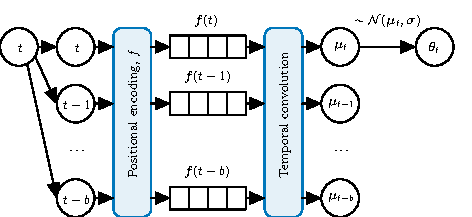
\includegraphics[labellifelongtrading=hyperpolicypolis]{img/thesis_plots_chapter_lifelong_trading.pdf}
    \caption{Graphical representation of the hyper-policy when queried at time $t$. 
    First, because the temporal convolution has a receptive field of length $b$, we append the last $b$ times to $t$ in the input fed to a positional encoding.
    The latter outputs a vector $\boldsymbol{f}(t)$ for each time. 
    These vectors are then fed to the temporal convolution which returns the mean $\boldsymbol{\mu}_k$ of each policy parameter $\boldsymbol\theta_k$ at time $k$.
    The last of these is the current policy parameter $\boldsymbol\theta_t$.}
    \label{fig:hyper_policy_polis}
\end{figure}


\subsection{Results}
\label{subsec:results_lifelong}

\noindent\textbf{Undelayed EUR-USD Trading.}\indent We report the results showing the cumulative return over time in \Cref{fig:trading_eurusd}.
In the upper figures, the hyperparameters are selected in the training set (2009-2012).  
Interestingly, for the period 2013-2016, the stationary policy achieves the best performance while POLIS has a very similar performance.
Recall that the stationary policy is only stationary in between re-training steps, however. 
The period 2017-2020 seems more complex as no approach yields a positive return. 
POLIS underperforms most of the baselines, yet not the stationary one.
In the lower figures, the hyperparameters are selected in the testing set (2013-2016 and 2017-2020 combined).  
In these tests, POLIS performs more similarly to other baselines, and no approach clearly outperforms the others. 

\begin{figure}[t]
    \centering
    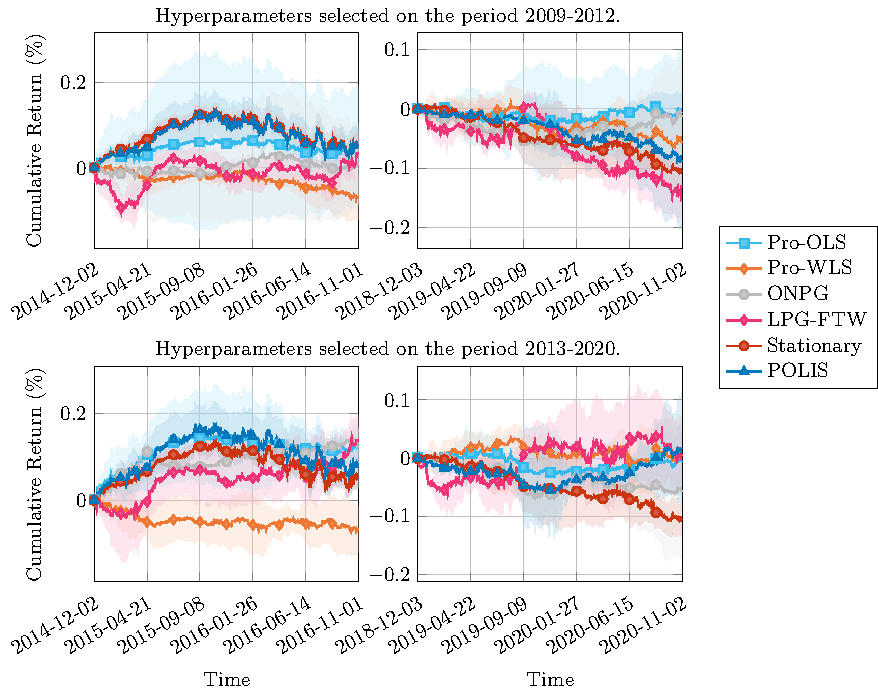
\includegraphics[labellifelongtradingtwo=polistradingeurusd]{img/thesis_plots_chapter_lifelong_trading_2.pdf}
    \caption{Cumulative return in percentage for the lifelong trading on the EUR-USD currency pair for two test datasets, 2013-2016 (left) and 2017-2020 (right). Note that only the target period is represented for each dataset.
    Hyper-parameters are selected for the period 2009-2012 (above) or 2013-2020 (below).
    The mean and one standard deviation shaded area are computed over 3 seeds.
    Markers correspond to the time of the re-train step.}
    \label{fig:trading_eurusd}
\end{figure}

\noindent\textbf{Undelayed Vasicek Trading.}\indent On this task, we have tested the set of hyperparameters selected for EUR-USD trading. 
The cumulative returns for the Vasicek trading problem are reported in \Cref{fig:trading_vasicek}. 
POLIS seems to be exploiting the clearer signals given by the synthetic asset more efficiently than the baselines. It achieves a higher final return and a smaller variance than other baselines. 
In particular, it clearly outperforms the stationary policy, which collects a negative return, most likely due to the fees.

As an extra experiment in this environment, we study the effect of POLIS' hyper-parameters $\lambda$ for the surrogate penalisation on the variance and $\beta$ for the number of steps ahead considered for the optimisation. 
For consider $\lambda\in[\![1, 100]\!]$ and of $\beta\in[\![2, 100]\!]$ \footnote{For $\beta=1$, the left term inside the \Renyi divergence in \Cref{lem:variance_bound} does not involve a mixture of distributions anymore and can be handled as in \cite{papini2019optimistic}.}. 
We are interested in studying how $\lambda$ and $\beta$ allow trading between the return and the standard deviation of the rewards.
The results, reported \Cref{fig:heatmap_vasicek}, suggest that a smaller $\beta$ generally yields a higher return, but at the cost of a
higher standard deviation. 
The effect of $\lambda$ on this trade-off is less clear.
However, as designed, this parameter allows one to control the standard deviation of the rewards.

\begin{figure}[t]
    \centering
    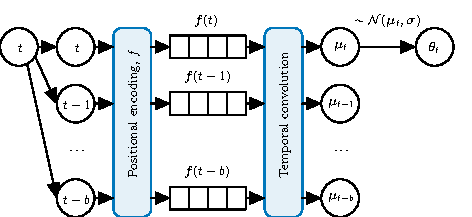
\includegraphics[labellifelongtrading=polisvasicektrading]{img/thesis_plots_chapter_lifelong_trading.pdf}
    \caption{Cumulative return in percentage for the lifelong trading on the Vasicek process. 
    The mean and one standard deviation shaded area are computed over 10 seeds.
    Markers correspond to the time of the re-train step.}
    \label{fig:trading_vasicek}
\end{figure}

\begin{figure*}[t]
\centering
\begin{subfigure}{.45\textwidth}
  \centering
  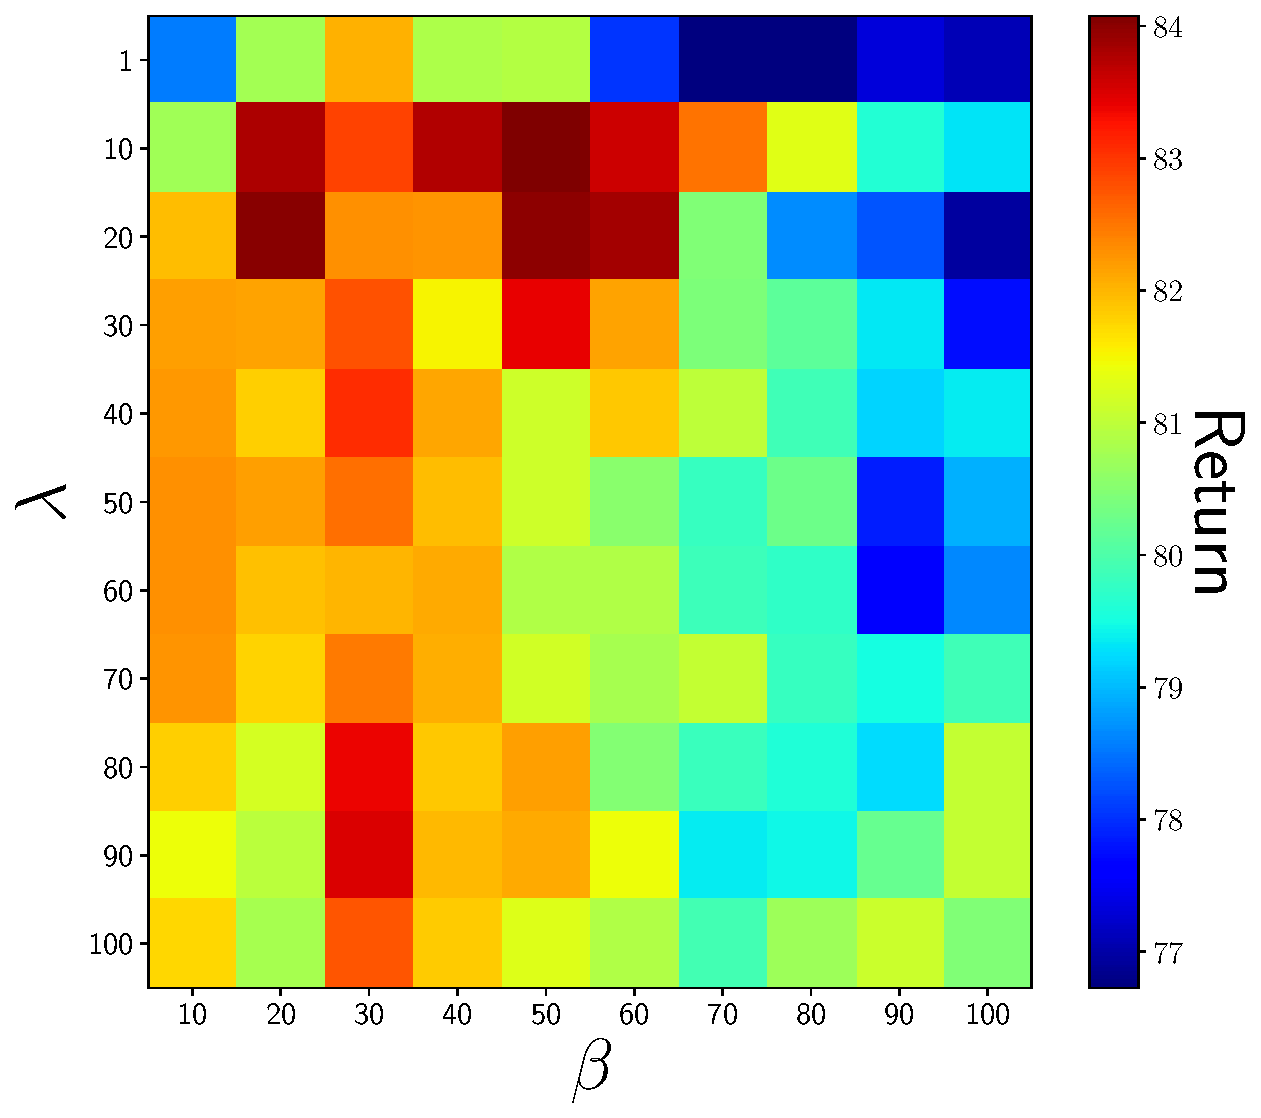
\includegraphics[width=\linewidth]{img/lifelong/vasicek_heatmap_return.pdf}
\end{subfigure}%
\hfill
\begin{subfigure}{.45\textwidth}
  \centering
  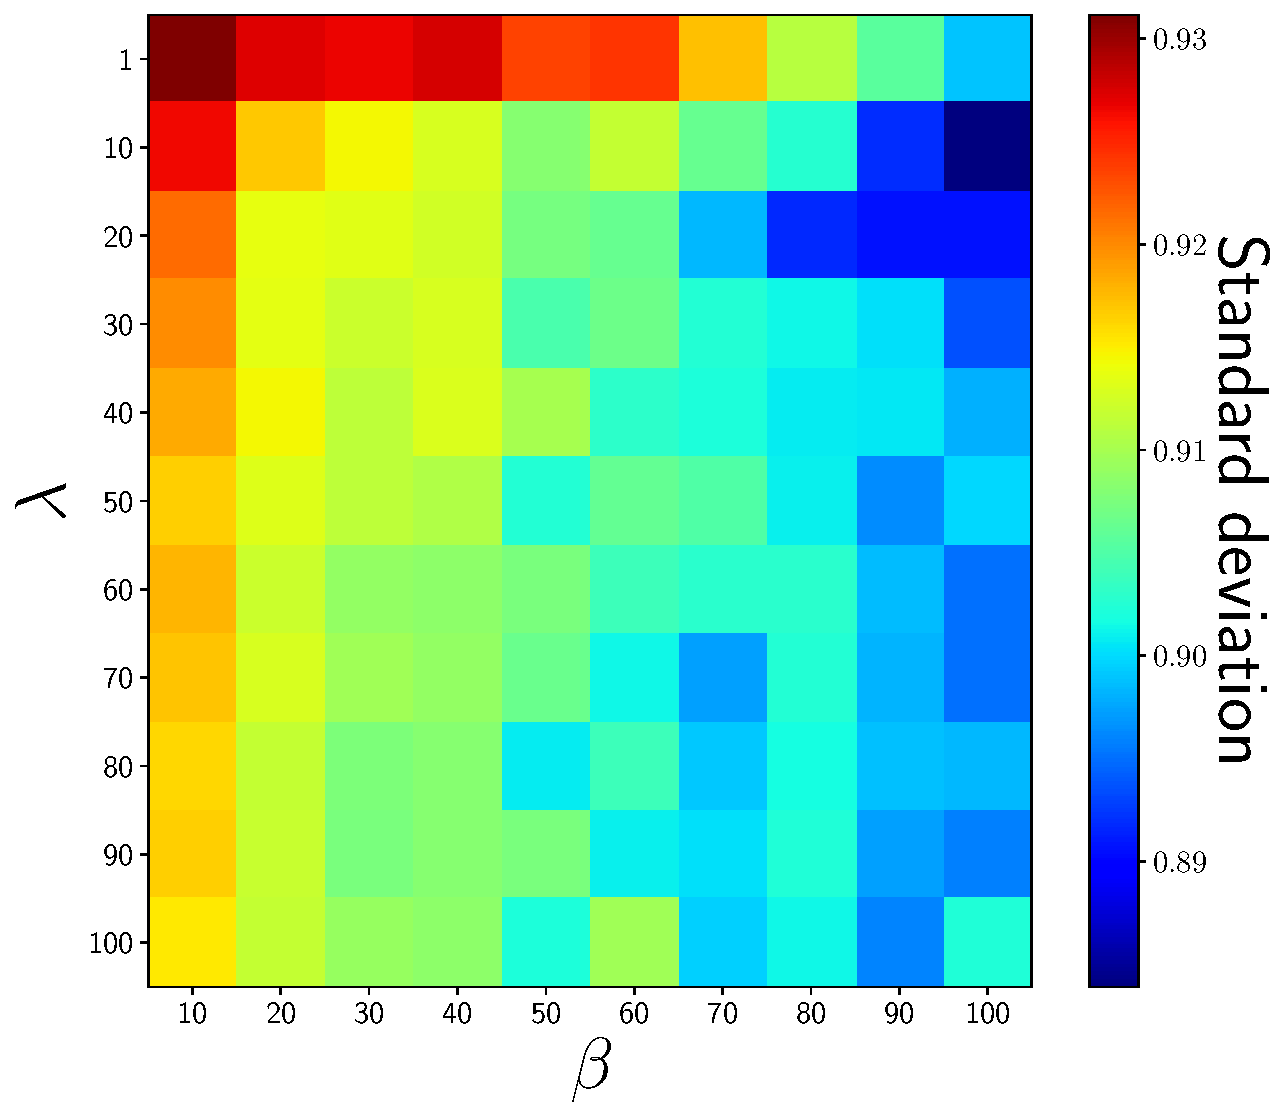
\includegraphics[width=\linewidth]{img/lifelong/vasicek_heatmap_standard_deviation.pdf}
\end{subfigure}%
\hfill
\captionof{figure}{Return (left) and standard deviation of the rewards (right) of POLIS on the Vasicek process as a function of $\lambda$
and $\beta$.}\label{fig:heatmap_vasicek}
\end{figure*}

\noindent\textbf{Undelayed Dam.}\indent We report the results of the experiment in \Cref{tab:exp_dam}. 
Surprisingly, out of all the baselines, the stationary hyper-policy obtains the best performance over the 3 inflows. 
Baselines, other than the stationary one, have lower returns and exhibit a tendency to have a higher standard deviation.
POLIS achieves much better returns than those baselines, including in terms of variance, and marches the stationary policy. 
This suggests that our approach is able to avoid extra non-stationarity in tasks where it is not needed. 

\begin{table}[t]
    \centering
    \begin{tabular}{l|lll}
          & \multicolumn{1}{c}{Inflow 1}       & \multicolumn{1}{c}{Inflow 2}        & \multicolumn{1}{c}{Inflow 3}       
        \\ \hline\hline
        Pro-OLS&$-2.6 \pm 0.4$&$-5.2 \pm 5.1$&$-3.8 \pm 0.7$\\
        Pro-WLS&$-5.5 \pm 4.3$&$-8.5 \pm 9.7$&$-8.4 \pm 4.2$\\
        ONPG&$-5.1 \pm 3.2$&$-1.4 \pm 0.2$&$-4.1 \pm 0.5$\\
        LPG-FTW&$-2.3 \pm 0.3$&$-11.9 \pm 8.6$&$-4.7 \pm 1.9$\\
        Stationary&$-2.2 \pm 0.1$&$-1.5 \pm 0.0$&$-3.2 \pm 0.2$\\
        POLIS&$-2.2 \pm 0.2$&$-1.5 \pm 0.0$&$-3.2 \pm 0.2$\\
    \end{tabular}
    \caption{Lifelong learning on the Dam environment for each of 3 inflow profiles. Mean return on the target period and standard deviation over 3 seeds. Reported results are divided by an order of $1e3$ for aesthetic.}\label{tab:exp_dam}
\end{table}


%\begin{table}[t]
%    \centering
%    \begin{tabular}{l|lll}
%          & \multicolumn{1}{c}{Inflow 1}       & \multicolumn{1}{c}{Inflow 2}        %& \multicolumn{1}{c}{Inflow 3}       
%        \\ \hline\hline
%        POLIS&$-1.3 \pm 1.0$&$-0.9 \pm 1.2$&$-4.0 \pm 3.2$\\
%        Stationary&$0.0 \pm 0.0$&$-5.3 \pm 0.4$&$-16.7 \pm 0.9$\\
%    \end{tabular}
%    \caption{Lifelong learning on the Dam environment for each of 3 inflow profile %with a longer number of steps between retrains. 
%    Mean return on the target period and standard deviation over 3 seeds. Reported %results are divided by an order of $1e3$ for aesthetic.}\label{tab:exp_dam_longer}
%\end{table}




\noindent\textbf{Delayed Vasicek Trading.}\indent The results are provided in \Cref{fig:delay_vasicek_trading}. 
As expected, as the delay grows, the performance of POLIS tarnishes. 
However, POLIS is quite robust to delay and, even for larger delays of 10 steps, obtains similar performances to the best-undelayed baselines of \Cref{fig:trading_vasicek}.

\begin{figure}[t]
    \centering
    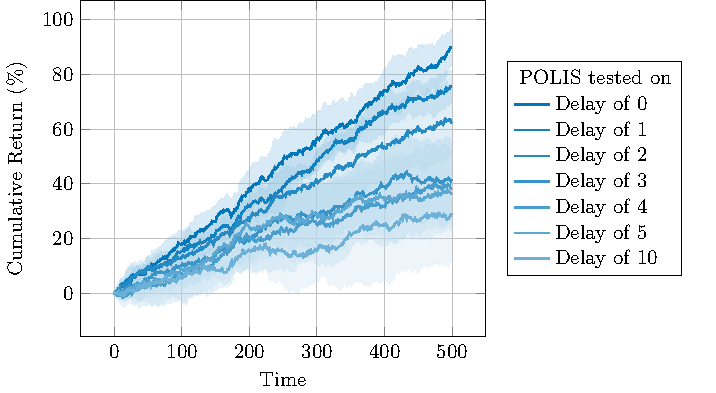
\includegraphics[labellifelongvasicek=polisdelayvasicek]{img/thesis_plots_chapter_lifelong_vasicek.pdf}
    \caption{Return obtained by running POLIS with an increasing delay on the Vasicek trading environment.}
    \label{fig:delay_vasicek_trading}
\end{figure}




\noindent\textbf{Delayed Dam.}\indent The results on the delayed test for the Dam are reported in \Cref{tab:exp_dam_delay}. 
The delay has a clear negative impact on performance. 
Surprisingly, the performance does not seem to drop further when going from a delay of 1 to a delay of 10 steps.  
We also note that the delay does not seem to have much impact on the variance, except for the second inflow profile.
The performance of POLIS, even for larger delays, is on par with the performance of the undelayed experts.

\begin{table}[t]
    \centering
    \begin{tabular}{l|llll}
          POLIS & \multicolumn{1}{c}{Undelayed} &
          \multicolumn{1}{c}{Delay of 1}       & \multicolumn{1}{c}{Delay of 5}        & \multicolumn{1}{c}{Delay of 10}       
        \\ \hline\hline
        Infow 1&$-2.2 \pm 0.2$&$-3.1 \pm 0.3$&$-3.2 \pm 0.2$&$-3.2 \pm 0.2$\\
        Infow 2&$-1.5 \pm 0.0$&$-1.4 \pm 0.2$&$-1.5 \pm 0.2$&$-1.5 \pm 0.3$\\
        Infow 3&$-3.2 \pm 0.2$&$-4.1 \pm 0.3$&$-4.1 \pm 0.2$&$-4.1 \pm 0.2$\\
    \end{tabular}
    \caption{Returns obtained by POLIS on the delayed Dam environment.
    Mean return on the target period and standard deviation over 3 seeds. 
    Reported results are divided by an order of $1e3$ for aesthetic.}\label{tab:exp_dam_delay}
\end{table}